\section{Ichsan Hizman Hardy(1174034)}
\subsection{Point Polyline dan Polygon}
\begin{enumerate}
	\item 
	\lstinputlisting{src/1/1174034/soal1.py}
	\begin{figure}[H]
		
\includegraphics[width=12cm]{figures/1174034/No1.JPG}
		\centering
		\caption{Point}
	\end{figure}
	
	\item 
	\lstinputlisting{src/1/1174034/No2.py}
	\begin{figure}[H]
		\includegraphics[width=12cm]{figures/1174034/No2.JPG}
		\centering
		\caption{Point}
	\end{figure}
	
	\item 
	\lstinputlisting{src/1/1174034/No3.py}
	\begin{figure}[H]
		\includegraphics[width=12cm]{figures/1174034/No3.JPG}
		\centering
		\caption{Point}
	\end{figure}
	
	\item 
	\lstinputlisting{src/1/1174034/No4.py}
	\begin{figure}[H]
		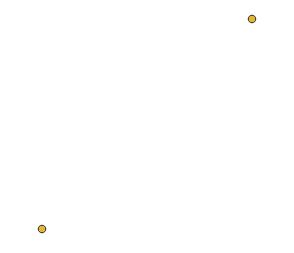
\includegraphics[width=12cm]{figures/1174042/No4.JPG}
		\centering
		\caption{Point}
	\end{figure}
	
	\item 
	\lstinputlisting{src/1/1174034/No5.py}
	\begin{figure}[H]
		
\includegraphics[width=12cm]{figures/1174034/No5.JPG}
		\centering
		\caption{Polyline}
	\end{figure}
	
	\item 
	\lstinputlisting{src/1/1174034/No6.py}
	\begin{figure}[H]
		\includegraphics[width=12cm]{figures/1174034/No6.JPG}
		\centering
		\caption{Poligon}
	\end{figure}
	
	\item 
	\lstinputlisting{src/1/1174034/No7.py}
	\begin{figure}[H]
		
\includegraphics[width=12cm]{figures/1174034/No7.JPG}
		\centering
		\caption{Polygon}
	\end{figure}
	
	\item 
	\lstinputlisting{src/1/1174034/No8.py}
	\begin{figure}[H]
		\includegraphics[width=12cm]{figures/1174034/No8.JPG}
		\centering
		\caption{Polygon}
	\end{figure}
	
	\item 
	\lstinputlisting{src/1/1174034/No9.py}
	\begin{figure}[H]
		\includegraphics[width=12cm]{figures/1174034/No9.JPG}
		\centering
		\caption{Polygon}
	\end{figure}
	
	\item 
	\lstinputlisting{src/1/1174034/No10.py}
	\begin{figure}[H]
		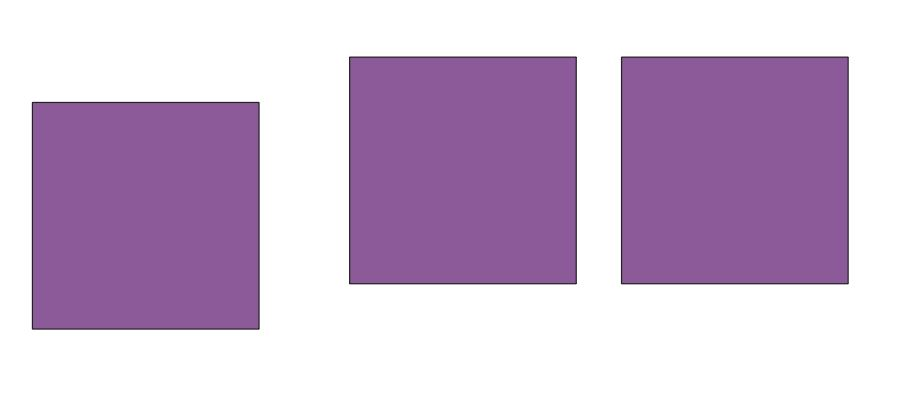
\includegraphics[width=12cm]{figures/1174034/No10.JPG}
		\centering
		\caption{Hasil mod saya yaitu 2 jadi yang saya kerjakan Bujursangkan yang berjum lah 4, Polygon}
	\end{figure}	
\end{enumerate}

\subsection{Link}
\href{https://youtu.be/4O3oxQESyjM\section{Liyana Majdah Rahma(1174039)}
\subsection{Point Polyline dan Polygon}
\begin{enumerate}
	\item 
	\lstinputlisting{src/1/1174039/soal1.py}
	\begin{figure}[H]
		
\includegraphics[width=12cm]{figures/1174042/No1.JPG}
		\centering
		\caption{Point}
	\end{figure}
	
	\item 
	\lstinputlisting{src/1/1174042/No2.py}
	\begin{figure}[H]
		\includegraphics[width=12cm]{figures/1174042/No2.JPG}
		\centering
		\caption{Point}
	\end{figure}
	
	\item 
	\lstinputlisting{src/1/1174042/No3.py}
	\begin{figure}[H]
		\includegraphics[width=12cm]{figures/1174042/No3.JPG}
		\centering
		\caption{Point}
	\end{figure}
	
	\item 
	\lstinputlisting{src/1/1174042/No4.py}
	\begin{figure}[H]
		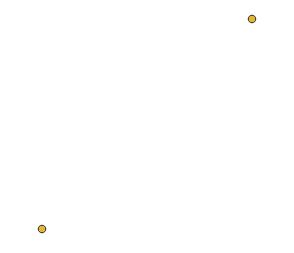
\includegraphics[width=12cm]{figures/1174042/No4.JPG}
		\centering
		\caption{Point}
	\end{figure}
	
	\item 
	\lstinputlisting{src/1/1174042/No5.py}
	\begin{figure}[H]
		
\includegraphics[width=12cm]{figures/1174042/No5.JPG}
		\centering
		\caption{Polyline}
	\end{figure}
	
	\item 
	\lstinputlisting{src/1/1174042/No6.py}
	\begin{figure}[H]
		\includegraphics[width=12cm]{figures/1174042/No6.JPG}
		\centering
		\caption{Poligon}
	\end{figure}
	
	\item 
	\lstinputlisting{src/1/1174042/No7.py}
	\begin{figure}[H]
		
\includegraphics[width=12cm]{figures/1174042/No7.JPG}
		\centering
		\caption{Polygon}
	\end{figure}
	
	\item 
	\lstinputlisting{src/1/1174042/No8.py}
	\begin{figure}[H]
		\includegraphics[width=12cm]{figures/1174042/No8.JPG}
		\centering
		\caption{Polygon}
	\end{figure}
	
	\item 
	\lstinputlisting{src/1/1174042/No9.py}
	\begin{figure}[H]
		\includegraphics[width=12cm]{figures/1174042/No9.JPG}
		\centering
		\caption{Polygon}
	\end{figure}
	
	\item 
	\lstinputlisting{src/1/1174042/No10.py}
	\begin{figure}[H]
		
\includegraphics[width=12cm]{figures/1174042/No10.JPG}
		\centering
		\caption{Hasil mod saya yaitu 2 jadi yang saya kerjakan Bujursangkan yang berjum lah 4, Polygon}
	\end{figure}	
\end{enumerate}

\subsection{Link}
\href{https://youtu.be/4O3oxQESyjM}{Youtube}}{Youtube}